% =============================================================================
% CAPÍTULO 2 - BLOQUE 2.2: FUNCIONAMIENTO Y TAXONOMÍA DE MODELOS DE EMBEDDINGS:
% DE LA ALINEACIÓN PROYECTADA A LAS TOPOLOGÍAS ASIMÉTRICAS BI/CROSS-ENCODER
% =============================================================================

\subsection{Funcionamiento y Taxonomía de Modelos de Embeddings Multimodales}
\label{subsec:taxonomia_modelos}

\subsubsection{Evolución Arquitectónica: De los Modelos Alineados (CLIP e ImageBind) a la Omnimodalidad Nativa}
\label{subsubsec:evolucion_clip_omnimodalidad}

El diseño de redes neuronales capaces de proyectar múltiples modalidades de datos dentro de un espacio métrico común ha atravesado tres generaciones claramente diferenciadas en la literatura científica reciente \cite{prajwal2025multimodal, qwen3_vl_emb2026}. Comprender las limitaciones estructurales de las dos primeras generaciones resulta indispensable para justificar la adopción de los modelos fundacionales omnimodales desarrollados entre finales de 2024 y 2026 \cite{gemini_emb2_docs, qwen3_vl_emb2026}.

Durante la primera etapa evolutiva, el estándar de la industria estuvo dominado por modelos de alineación dual o múltiple como \textbf{CLIP} (\textit{Contrastive Language-Image Pre-training}, desarrollado por OpenAI) e \textbf{ImageBind} (desarrollado por Meta) \cite{prajwal2025multimodal}. Estas arquitecturas lograron un hito fundacional al demostrar que era posible entrenar codificadores separados (un codificador visual y un codificador textual) mediante aprendizaje contrastivo para alinear texto e imágenes estáticas (y, en casos puntuales como ImageBind, señales de audio) dentro de un mismo hiperplano vectorial \cite{prajwal2025multimodal}. Sin embargo, cuando estas arquitecturas de primera generación se aplicaban a la recuperación de información en secuencias de vídeo de larga duración, presentaban una limitación insalvable: carecían de una comprensión temporal nativa e integrada \cite{prajwal2025multimodal, rethinking_long_video2026}. Como consecuencia, la arquitectura tradicional obligaba a descomponer artificialmente el flujo multimedia: los ingenieros debían extraer y procesar los fotogramas de manera aislada, emplear modelos de transcripción fonética independientes para la pista de audio (como Whisper) y terminar indexando toda la información resultante como texto plano \cite{video_rag2024}. Este flujo fragmentado no solo resultaba computacionalmente torpe, sino que destruía el contexto temporal y la sincronía entre la acción visual y el suceso acústico \cite{prajwal2025multimodal}.

Una segunda generación de transición surgió a principios de 2025 con propuestas académicas como \textbf{VLM2Vec} y arquitecturas de interacción tardía como \textbf{ColQwen} \cite{prajwal2025multimodal}. El mérito científico de \textit{VLM2Vec} (construido sobre modelos de lenguaje visuales genéricos como LLaVA y Phi) consistió en demostrar empíricamente cómo transformar un Modelo de Lenguaje Visual (\textit{Vision-Language Model}, VLM) originalmente concebido para la generación autorregresiva de texto en un extractor masivo de \textit{embeddings} multimodales para texto, imagen y vídeo. En paralelo, sistemas como \textit{ColQwen} demostraron que era posible eliminar los motores OCR intermedios proyectando directamente las teselas visuales hacia el espacio latente del lenguaje \cite{prajwal2025multimodal}.

Finalmente, entre finales de 2024 y el primer trimestre de 2026 se consolida la tercera generación: los \textbf{Modelos de Embedding Omnimodales (\textit{Omni-modality})} \cite{gemini_emb2_docs, qwen3_vl_emb2026}. Liderados en el ámbito comercial por \textbf{Gemini Embedding 2} (Google) y en el ecosistema de pesos abiertos por la familia \textbf{Qwen3-VL-Embedding} (Alibaba) y \textbf{EmbeddingGemma 2} (Google DeepMind), estos sistemas han sido diseñados desde su pre-entrenamiento para ingerir de forma nativa texto, imágenes, secuencias de vídeo, pistas de audio y documentos estructurados (archivos PDF) proyectándolos directamente en un único vector denso sin pasos de traducción textual intermedios \cite{gemini_emb2_docs, qwen3_vl_emb2026}.

La Figura~\ref{fig:evolucion_generaciones_embeddings} sintetiza gráficamente la transición arquitectónica a través de estas tres generaciones de modelos de representación.

\begin{figure}[htbp]
\centering
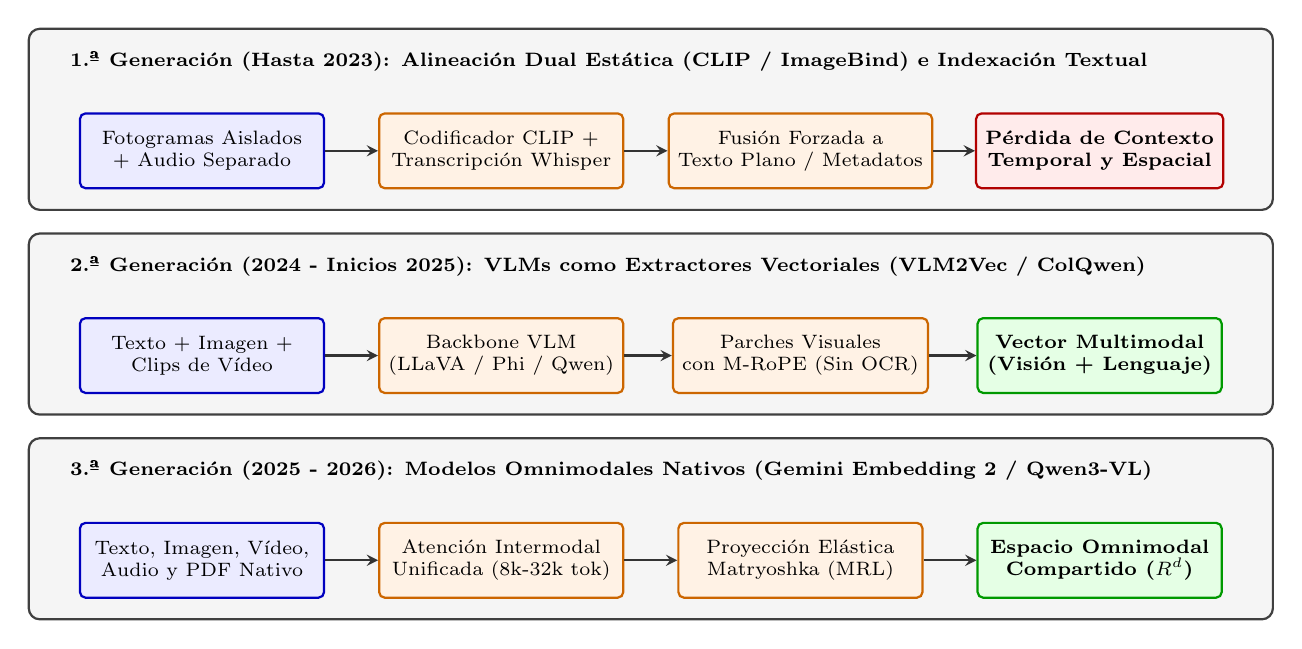
\begin{tikzpicture}[
    node distance=0.5cm and 0.6cm,
    genbox/.style={rectangle, draw=black!75, fill=gray!8, thick, minimum width=15.8cm, minimum height=2.3cm, rounded corners=4pt},
    modbox/.style={rectangle, draw=blue!75!black, fill=blue!8, thick, minimum width=3.1cm, minimum height=0.95cm, align=center, font=\scriptsize, rounded corners=2pt},
    procbox/.style={rectangle, draw=orange!80!black, fill=orange!10, thick, minimum width=3.1cm, minimum height=0.95cm, align=center, font=\scriptsize, rounded corners=2pt},
    outbox/.style={rectangle, draw=green!60!black, fill=green!10, thick, minimum width=3.1cm, minimum height=0.95cm, align=center, font=\scriptsize\bfseries, rounded corners=2pt},
    arrow/.style={-stealth, thick, draw=black!80}
]
% Generación 1
\node[genbox] (g1) at (0, 5.2) {};
\node[font=\scriptsize\bfseries, anchor=north west] at (-7.5, 6.18) {1.ª Generación (Hasta 2023): Alineación Dual Estática (CLIP / ImageBind) e Indexación Textual};
\node[modbox] (g1_in) at (-5.7, 4.80) {Fotogramas Aislados\\+ Audio Separado};
\node[procbox] (g1_proc) at (-1.9, 4.80) {Codificador CLIP +\\Transcripción Whisper};
\node[procbox] (g1_txt) at (1.9, 4.80) {Fusión Forzada a\\Texto Plano / Metadatos};
\node[outbox, draw=red!70!black, fill=red!8] (g1_out) at (5.7, 4.80) {Pérdida de Contexto\\Temporal y Espacial};
\draw[arrow] (g1_in) -- (g1_proc);
\draw[arrow] (g1_proc) -- (g1_txt);
\draw[arrow] (g1_txt) -- (g1_out);

% Generación 2
\node[genbox] (g2) at (0, 2.6) {};
\node[font=\scriptsize\bfseries, anchor=north west] at (-7.5, 3.58) {2.ª Generación (2024 - Inicios 2025): VLMs como Extractores Vectoriales (VLM2Vec / ColQwen)};
\node[modbox] (g2_in) at (-5.7, 2.20) {Texto + Imagen +\\Clips de Vídeo};
\node[procbox] (g2_proc) at (-1.9, 2.20) {Backbone VLM\\(LLaVA / Phi / Qwen)};
\node[procbox] (g2_mrope) at (1.9, 2.20) {Parches Visuales\\con M-RoPE (Sin OCR)};
\node[outbox] (g2_out) at (5.7, 2.20) {Vector Multimodal\\(Visión + Lenguaje)};
\draw[arrow] (g2_in) -- (g2_proc);
\draw[arrow] (g2_proc) -- (g2_mrope);
\draw[arrow] (g2_mrope) -- (g2_out);

% Generación 3
\node[genbox] (g3) at (0, 0.0) {};
\node[font=\scriptsize\bfseries, anchor=north west] at (-7.5, 0.98) {3.ª Generación (2025 - 2026): Modelos Omnimodales Nativos (Gemini Embedding 2 / Qwen3-VL)};
\node[modbox] (g3_in) at (-5.7, -0.40) {Texto, Imagen, Vídeo,\\Audio y PDF Nativo};
\node[procbox] (g3_proc) at (-1.9, -0.40) {Atención Intermodal\\Unificada (8k-32k tok)};
\node[procbox] (g3_mrl) at (1.9, -0.40) {Proyección Elástica\\Matryoshka (MRL)};
\node[outbox] (g3_out) at (5.7, -0.40) {Espacio Omnimodal\\Compartido ($\mathbb{R}^d$)};
\draw[arrow] (g3_in) -- (g3_proc);
\draw[arrow] (g3_proc) -- (g3_mrl);
\draw[arrow] (g3_mrl) -- (g3_out);
\end{tikzpicture}
\caption{Evolución taxonómica de los modelos de representación vectorial: desde la alineación estática dependiente de transcripción textual (CLIP/Whisper) hasta los modelos omnimodales nativos de tercera generación capaces de proyectar texto, imagen, vídeo, audio y PDF en un único clúster topológico \cite{prajwal2025multimodal, gemini_emb2_docs, qwen3_vl_emb2026}.}
\label{fig:evolucion_generaciones_embeddings}
\end{figure}

\subsubsection{Tokenización Visual, Codificación M-RoPE y Agregación Temporal de Fotogramas}
\label{subsubsec:tokenizacion_mrope_agregacion}

A nivel interno, el funcionamiento de un modelo de \textit{embedding} multimodal contemporáneo se apoya en la unificación de la representación de entrada mediante teselas o parches (\textit{visual patches}) procesados por arquitecturas inspiradas en \textit{Vision Transformers} (ViT) \cite{prajwal2025multimodal}. Cuando el sistema recibe un fotograma de vídeo o una página de un documento visual a su resolución nativa, divide la matriz bidimensional de píxeles en una secuencia de sub-bloques que se proyectan linealmente como \textit{tokens} visuales dentro de la misma secuencia de entrada que los \textit{tokens} léxicos del texto \cite{prajwal2025multimodal}.

Para evitar que esta linealización destruya la geometría bidimensional de la imagen o la secuencia temporal del vídeo, las arquitecturas modernas incorporan \textbf{\textit{Multimodal Rotary Position Embeddings}} (\textbf{M-RoPE}) \cite{prajwal2025multimodal}. M-RoPE codifica directamente la información posicional bidimensional y temporal sobre las representaciones latentes de cada parche visual, lo que resulta determinante al procesar fotogramas de vídeo con resoluciones variables, garantizando que las relaciones espaciales entre los objetos visuales (como un bloque de código fuente en una esquina de la pantalla y el ponente en el lado opuesto) queden alineadas en el mismo espacio vectorial que los \textit{tokens} del Modelo de Lenguaje Grande (LLM) subyacente \cite{prajwal2025multimodal}.

Un aspecto arquitectónico fundamental en la vectorización de fragmentos de vídeo (\texttt{VideoChunk}) radica en el mecanismo de \textbf{agregación temporal de múltiples fotogramas} \cite{gemini_emb2_docs}. Cuando un algoritmo de segmentación semántica adaptativa (como \textit{Video-RAC}) extrae tres fotogramas representativos de un plano (el fotograma inicial, el de máxima entropía visual y el fotograma final), existen dos formas opuestas de invocar al modelo fundacional \cite{video_rac2025, gemini_emb2_docs}:
\begin{enumerate}
    \item \textbf{Codificación Independiente por Fotograma (Incorrecta para cohesión de \textit{chunk}):} Si los tres fotogramas se envían a la API como tres objetos de contenido separados, el modelo genera tres vectores independientes ($\mathbf{v}_1, \mathbf{v}_2, \mathbf{v}_3 \in \mathbb{R}^d$). Esto triplica el coste de almacenamiento en la base de datos vectorial y obliga a realizar promedios heurísticos posteriores que diluyen la semántica temporal del plano.
    \item \textbf{Agregación Nativa en un Único Objeto \texttt{Content} (Estado del Arte):} En arquitecturas como \textit{Gemini Embedding 2}, al codificar los tres fotogramas clave en memoria (por ejemplo, en formato JPEG) e inyectarlos como múltiples objetos \texttt{Part} dentro de una única estructura \texttt{types.Content}, el mecanismo de atención interna del modelo evalúa conjuntamente la evolución entre los tres instantes y devuelve \textbf{un único \textit{embedding} denso agregado} $\mathbf{v}_{\text{chunk}} \in \mathbb{R}^d$ que sintetiza el significado completo del evento \cite{gemini_emb2_docs}.
\end{enumerate}

La Figura~\ref{fig:agregacion_temporal_content} ilustra cómo la agrupación de múltiples partes multimedia dentro de un mismo contenedor \texttt{Content} permite condensar la dinámica del fragmento temporal en un único punto del espacio latente.

\begin{figure}[htbp]
\centering
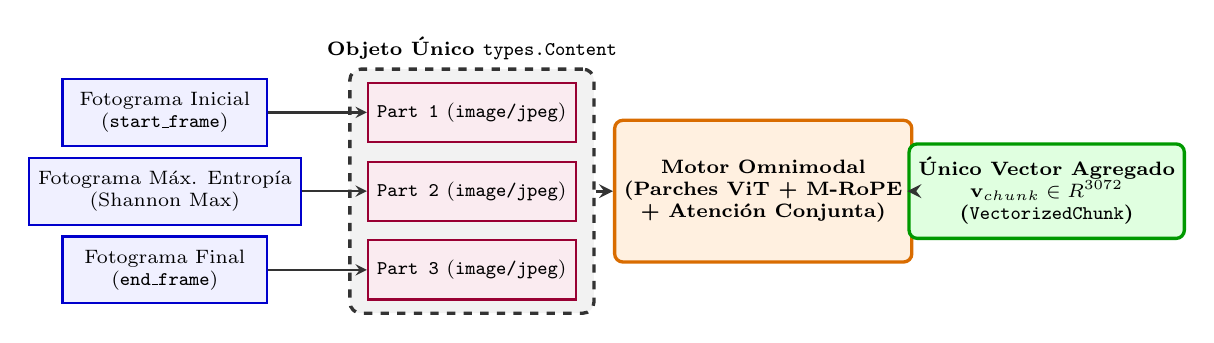
\begin{tikzpicture}[
    node distance=0.6cm and 0.8cm,
    framebox/.style={rectangle, draw=blue!80!black, fill=blue!6, thick, minimum width=2.6cm, minimum height=0.85cm, align=center, font=\scriptsize},
    partbox/.style={rectangle, draw=purple!80!black, fill=purple!8, thick, minimum width=2.4cm, minimum height=0.75cm, align=center, font=\scriptsize},
    contentbox/.style={rectangle, draw=black!80, fill=gray!10, very thick, dashed, minimum width=3.1cm, minimum height=3.1cm, rounded corners=4pt},
    modelbox/.style={rectangle, draw=orange!85!black, fill=orange!12, very thick, minimum width=3.0cm, minimum height=1.8cm, align=center, font=\scriptsize\bfseries, rounded corners=3pt},
    vecbox/.style={rectangle, draw=green!60!black, fill=green!12, very thick, minimum width=3.0cm, minimum height=1.2cm, align=center, font=\scriptsize\bfseries, rounded corners=3pt},
    arrow/.style={-stealth, thick, draw=black!80}
]
% Fotogramas extraídos del VideoChunk
\node[framebox] (f1) at (-5.2, 1.0) {Fotograma Inicial\\(\texttt{start\_frame})};
\node[framebox] (f2) at (-5.2, 0.0) {Fotograma Máx. Entropía\\(Shannon Max)};
\node[framebox] (f3) at (-5.2, -1.0) {Fotograma Final\\(\texttt{end\_frame})};

% Contenedor único types.Content
\node[contentbox] (cont) at (-1.3, 0.0) {};
\node[font=\scriptsize\bfseries, anchor=south] at (-1.3, 1.55) {Objeto Único \texttt{types.Content}};
\node[partbox] (p1) at (-1.3, 1.0) {\texttt{Part 1} (\texttt{image/jpeg})};
\node[partbox] (p2) at (-1.3, 0.0) {\texttt{Part 2} (\texttt{image/jpeg})};
\node[partbox] (p3) at (-1.3, -1.0) {\texttt{Part 3} (\texttt{image/jpeg})};

% Modelo y salida
\node[modelbox] (mod) at (2.4, 0.0) {Motor Omnimodal\\(Parches ViT + M-RoPE\\+ Atención Conjunta)};
\node[vecbox] (vec) at (6.0, 0.0) {Único Vector Agregado\\$\mathbf{v}_{\text{chunk}} \in \mathbb{R}^{3072}$\\(\texttt{VectorizedChunk})};

\draw[arrow] (f1) -- (p1);
\draw[arrow] (f2) -- (p2);
\draw[arrow] (f3) -- (p3);
\draw[arrow, very thick] (cont.east) -- (mod.west);
\draw[arrow, very thick] (mod.east) -- (vec.west);
\end{tikzpicture}
\caption{Mecanismo de agregación intermodal en \textit{Gemini Embedding 2}: los tres fotogramas representativos de un \texttt{VideoChunk} se empaquetan como objetos \texttt{Part} individuales dentro de un único contenedor \texttt{types.Content}, permitiendo que el modelo fusione la información temporal y devuelva un único vector denso por fragmento \cite{gemini_emb2_docs, video_rac2025}.}
\label{fig:agregacion_temporal_content}
\end{figure}

\subsubsection{Arquitecturas de Doble Torre (\textit{Bi-Encoder}) para Recuperación Masiva Pre-computada}
\label{subsubsec:arquitectura_bi_encoder}

En el diseño de sistemas de recuperación de información sobre grandes volúmenes de vídeo, la primera etapa del procesamiento recae sobre los modelos con \textbf{arquitectura de Doble Torre (\textit{Bi-Encoder})}, representados en el estado del arte por sistemas como \textit{Gemini Embedding 2}, \textit{Qwen3-VL-Embedding} (en sus variantes de 2B y 8B de parámetros) y \textit{EmbeddingGemma 2} \cite{gemini_emb2_docs, qwen3_vl_emb2026}.

La característica definitoria de un \textit{Bi-Encoder} es que procesa de manera completamente independiente el documento multimedia candidato $D_i$ (un fragmento de vídeo, una imagen o una pista de audio) y la consulta textual del usuario $Q$ \cite{learnopencv_qwen3, qwen3_vl_emb2026}. Matemáticamente, sean $f_{\theta}^{\text{doc}}$ y $f_{\theta}^{\text{query}}$ las funciones de proyección de ambas torres (que en los modelos fundacionales modernos suelen compartir los mismos pesos neuronales $\theta$, diferenciándose únicamente por el prefijo de instrucción de entrada), según se define en la Ecuación~\eqref{eq:bi_encoder_proyeccion} \cite{hf_train_multimodal2026}:

\begin{equation}
\mathbf{v}_i = f_{\theta}^{\text{doc}}(D_i) \in \mathbb{R}^d, \qquad \mathbf{q} = f_{\theta}^{\text{query}}(P_{\text{task}} \oplus Q) \in \mathbb{R}^d
\label{eq:bi_encoder_proyeccion}
\end{equation}

donde $P_{\text{task}}$ representa un prefijo corto de instrucción de tarea que se antepone exclusivamente a las entradas de texto para orientar la consulta en el espacio latente (técnica empleada explícitamente en modelos como \textit{EmbeddingGemma 2} y \textit{Qwen3-VL-Embedding}, pero que no se aplica a las imágenes, vídeos ni audios) \cite{qwen3_vl_emb2026}.

Esta independencia algebraica entre $\mathbf{v}_i$ y $\mathbf{q}$ constituye la piedra angular de la escalabilidad industrial por tres motivos fundamentales \cite{learnopencv_qwen3}:
\begin{enumerate}
    \item \textbf{Indexación Pasiva \textit{Offline}:} Permite pre-computar una sola vez los vectores $\mathbf{v}_i$ de un archivo histórico compuesto por millones de horas de vídeo y almacenarlos pasivamente en bases de datos vectoriales indexadas estáticamente como Qdrant o Milvus \cite{learnopencv_qwen3}.
    \item \textbf{Complejidad de Inferencia Constante respecto al Modelo:} Cuando el usuario introduce una búsqueda en lenguaje natural en tiempo de ejecución, la red neuronal profunda solo se ejecuta una vez para codificar la consulta $\mathbf{q}$ \cite{learnopencv_qwen3}.
    \item \textbf{Maximización de la Tasa de Recuerdo (\textit{Recall}) a Escala de Petabytes:} La recuperación se reduce a comparar el vector $\mathbf{q}$ recién generado contra los millones de vectores pre-computados mediante operaciones vectoriales ultrarrápidas (como el producto punto escalar o la similitud del coseno), logrando tiempos de respuesta de milisegundos \cite{learnopencv_qwen3, qwen3_vl_emb2026}.
\end{enumerate}

\subsubsection{Arquitecturas de Torre Única (\textit{Cross-Encoder / Reranker}) y Atención Cruzada}
\label{subsubsec:arquitectura_cross_encoder}

A pesar de su extraordinaria velocidad, los modelos \textit{Bi-Encoder} sufren una limitación estructural derivada de comprimir todo un fragmento de vídeo en un único vector estático $\mathbf{v}_i$ sin conocer de antemano qué preguntará el usuario \cite{learnopencv_qwen3, qwen3_vl_emb2026}. Al no existir interacción directa entre los \textit{tokens} de la consulta y los parches visuales del vídeo durante la codificación, ciertos detalles composicionales finos o textos pequeños en pantalla pueden quedar diluidos dentro de la representación global.

Para resolver esta pérdida de precisión sin sacrificar la escalabilidad, el estado del arte introduce los modelos con \textbf{arquitectura de Torre Única (\textit{Cross-Encoder})}, denominados operativamente \textbf{\textit{Rerankers}} (reordenadores) o verificadores visuales de segunda etapa, entre los que destacan \textbf{Qwen3-VL-Reranker} (en variantes de 2B y 8B) y el uso de modelos ligeros de visión-lenguaje como \textbf{Gemini 1.5 Flash Lite} o \textbf{Gemini Flash 3.5} en tareas de validación visual \cite{learnopencv_qwen3, qwen3_vl_emb2026}.

A diferencia del \textit{Bi-Encoder}, un \textit{Cross-Encoder} no genera vectores independientes ni permite pre-computar representaciones de los vídeos \cite{learnopencv_qwen3}. En su lugar, recibe simultáneamente en una única secuencia concatenada la consulta del usuario $Q$ y el fragmento multimedia candidato $D_k$, procesándolos conjuntamente a través de todas las capas de \textbf{Atención Cruzada (\textit{Cross-Attention})} del \textit{Transformer}, como se formula en la Ecuación~\eqref{eq:cross_encoder_score} \cite{learnopencv_qwen3, qwen3_vl_emb2026}:

\begin{equation}
s_k = g_{\phi}(Q, D_k) = \sigma\!\left(\mathbf{W}_{\text{head}} \cdot \text{CrossAttention}_{\phi}\!\left([\text{Tokens}(Q); \, \text{Patches}(D_k)]\right)\right) \in [0, 1]
\label{eq:cross_encoder_score}
\end{equation}

Mediante el mecanismo de \textit{Cross-Attention}, cada \textit{token} de la pregunta del usuario (por ejemplo, la palabra \textit{``diccionarios''}) atiende directamente a cada parche visual específico de los fotogramas del candidato $D_k$ (por ejemplo, la región de la pantalla donde aparece escrito el código \texttt{dict \{"name": "Brais"\}}). Finalmente, como refleja el Cuadro de especificaciones de la familia Qwen3-VL, el \textit{Cross-Encoder} no devuelve un vector de \textit{embedding}, sino una \textbf{probabilidad discreta en el rango $[0, 1]$} (o un veredicto de validación visual) que cuantifica la relevancia exacta del candidato respecto a la consulta \cite{qwen3_vl_emb2026}.

La Figura~\ref{fig:bi_encoder_vs_cross_encoder} contrasta detalladamente la topología interna de un \textit{Bi-Encoder} frente a la de un \textit{Cross-Encoder} \cite{learnopencv_qwen3, qwen3_vl_emb2026}.

\begin{figure}[htbp]
\centering
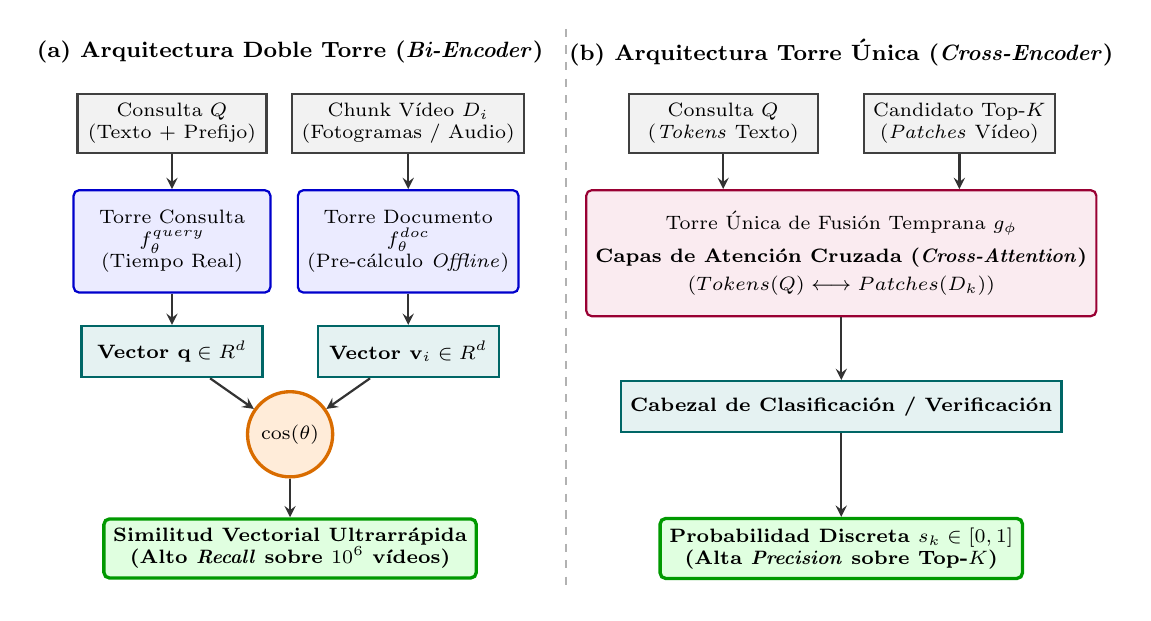
\begin{tikzpicture}[
    node distance=0.5cm and 0.7cm,
    tower/.style={rectangle, draw=blue!80!black, fill=blue!8, thick, minimum width=2.5cm, minimum height=1.3cm, align=center, font=\scriptsize, rounded corners=2pt},
    crosstower/.style={rectangle, draw=purple!80!black, fill=purple!8, thick, minimum width=5.4cm, minimum height=1.6cm, align=center, font=\scriptsize, rounded corners=2pt},
    inputbox/.style={rectangle, draw=black!75, fill=gray!10, thick, minimum width=2.4cm, minimum height=0.75cm, align=center, font=\scriptsize},
    vecnode/.style={rectangle, draw=teal!80!black, fill=teal!10, thick, minimum width=2.3cm, minimum height=0.65cm, align=center, font=\scriptsize\bfseries},
    opnode/.style={circle, draw=orange!85!black, fill=orange!15, very thick, minimum size=0.9cm, align=center, font=\scriptsize\bfseries},
    scorebox/.style={rectangle, draw=green!60!black, fill=green!12, very thick, minimum width=3.2cm, minimum height=0.75cm, align=center, font=\scriptsize\bfseries, rounded corners=2pt},
    arrow/.style={-stealth, thick, draw=black!80}
]
% --- LADO IZQUIERDO: BI-ENCODER ---
\node[font=\bfseries\footnotesize] at (-3.5, 4.0) {(a) Arquitectura Doble Torre (\textit{Bi-Encoder})};

\node[inputbox] (bi_q) at (-5.0, 3.1) {Consulta $Q$\\(Texto + Prefijo)};
\node[inputbox] (bi_d) at (-2.0, 3.1) {Chunk Vídeo $D_i$\\(Fotogramas / Audio)};

\node[tower] (t_q) at (-5.0, 1.6) {Torre Consulta\\$f_{\theta}^{\text{query}}$\\(Tiempo Real)};
\node[tower] (t_d) at (-2.0, 1.6) {Torre Documento\\$f_{\theta}^{\text{doc}}$\\(Pre-cálculo \textit{Offline})};

\node[vecnode] (v_q) at (-5.0, 0.2) {Vector $\mathbf{q} \in \mathbb{R}^d$};
\node[vecnode] (v_d) at (-2.0, 0.2) {Vector $\mathbf{v}_i \in \mathbb{R}^d$};

\node[opnode] (cos) at (-3.5, -0.85) {$\cos(\theta)$};
\node[scorebox] (bi_out) at (-3.5, -2.30) {Similitud Vectorial Ultrarrápida\\(Alto \textit{Recall} sobre $10^6$ vídeos)};

\draw[arrow] (bi_q) -- (t_q);
\draw[arrow] (bi_d) -- (t_d);
\draw[arrow] (t_q) -- (v_q);
\draw[arrow] (t_d) -- (v_d);
\draw[arrow] (v_q) -- (cos);
\draw[arrow] (v_d) -- (cos);
\draw[arrow] (cos) -- (bi_out);

% Línea divisoria central
\draw[dashed, gray!60, thick] (0.0, 4.3) -- (0.0, -2.85);

% --- LADO DERECHO: CROSS-ENCODER ---
\node[font=\bfseries\footnotesize] at (3.5, 4.0) {(b) Arquitectura Torre Única (\textit{Cross-Encoder})};

\node[inputbox] (cr_q) at (2.0, 3.1) {Consulta $Q$\\(\textit{Tokens} Texto)};
\node[inputbox] (cr_d) at (5.0, 3.1) {Candidato Top-$K$\\(\textit{Patches} Vídeo)};

\node[crosstower] (cr_t) at (3.5, 1.45) {Torre Única de Fusión Temprana $g_{\phi}$\\[4pt]
\textbf{Capas de Atención Cruzada (\textit{Cross-Attention})}\\[2pt]
($\text{Tokens}(Q) \longleftrightarrow \text{Patches}(D_k)$)};

\node[vecnode, minimum width=4.2cm] (cr_head) at (3.5, -0.5) {Cabezal de Clasificación / Verificación};
\node[scorebox] (cr_out) at (3.5, -2.30) {Probabilidad Discreta $s_k \in [0, 1]$\\(Alta \textit{Precision} sobre Top-$K$)};

\draw[arrow] (cr_q) -- (cr_q |- cr_t.north);
\draw[arrow] (cr_d) -- (cr_d |- cr_t.north);
\draw[arrow] (cr_t) -- (cr_head);
\draw[arrow] (cr_head) -- (cr_out);
\end{tikzpicture}
\caption{Comparativa estructural entre (a) un \textit{Bi-Encoder} de doble torre que codifica consulta y vídeo de forma independiente para indexación pasiva en bases de datos vectoriales, y (b) un \textit{Cross-Encoder} (\textit{Reranker}) que aplica atención cruzada conjunta sobre el subconjunto de candidatos recuperados \cite{learnopencv_qwen3, qwen3_vl_emb2026}.}
\label{fig:bi_encoder_vs_cross_encoder}
\end{figure}

\subsubsection{Eficiencia Escalable: El Paradigma de Búsqueda Asimétrica en Dos Etapas (Regla 99\% / 1\%)}
\label{subsubsec:busqueda_asimetrica_dos_etapas}

El resurgimiento y perfeccionamiento de la dualidad entre \textit{Bi-Encoders} (para recuperación inicial) y \textit{Cross-Encoders} o verificadores VLM (para refinamiento) responde directamente a los límites físicos de energía, latencia y procesamiento de hardware en sistemas de vídeo a gran escala \cite{learnopencv_qwen3, rethinking_long_video2026}. Computar de forma cruzada cada búsqueda del usuario contra terabytes de fragmentos de vídeo utilizando modelos generativos masivos (como intentar emplear un modelo tipo Llama-Vision o Gemini Pro para comparar fotograma a fotograma todo un repositorio) resulta técnica y financieramente inasumible \cite{learnopencv_qwen3}.

Para resolver esta dicotomía, el estado del arte de 2026 establece una \textbf{aproximación asimétrica radical en dos etapas} conocida como la regla del $99\% / 1\%$ \cite{learnopencv_qwen3, qwen3_vl_emb2026}:
\begin{itemize}
    \item \textbf{Primera Etapa - Filtrado Masivo del 99\% (\textit{Bi-Encoder} + Base de Datos Vectorial):} Se delega el $99\%$ del descarte de datos a una vectorización paralela, densa e independiente (empleando modelos como \textit{Gemini Embedding 2} o \textit{Qwen3-VL-Embedding}) almacenada en un motor vectorial como Qdrant \cite{gemini_emb2_docs, qwen3_vl_emb2026}. Ante una consulta del usuario, la búsqueda inicial se resuelve mediante un cálculo vectorial de similitud del coseno sobre índices estáticos, reduciendo instantáneamente miles de fragmentos a una lista acotada de los $K$ mejores candidatos (por ejemplo, $\text{Top-}K = 5$ o $\text{Top-}K = 20$) \cite{learnopencv_qwen3}.
    \item \textbf{Segunda Etapa - Refinamiento Intensivo del 1\% (\textit{Cross-Encoder} / Verificación Visual):} El cómputo pesado, iterativo y apoyado en mecanismos de atención cruzada se reserva exclusivamente para ese $1\%$ de resultados candidatos recuperados en la primera fase \cite{learnopencv_qwen3}. En esta etapa, bien un modelo específico de reordenación (\textit{Qwen3-VL-Reranker}) recalcula la probabilidad exacta de coincidencia $[0, 1]$, o bien un verificador visual ligero (\textit{Gemini 1.5 Flash Lite} / \textit{Gemini Flash 3.5}) inspecciona los fotogramas del \textit{chunk} candidato para descartar falsos positivos antes de presentar los intervalos de tiempo (\texttt{start\_time} - \texttt{end\_time}) definitivos al usuario \cite{learnopencv_qwen3, qwen3_vl_emb2026}.
\end{itemize}

\begin{figure}[htbp]
\centering
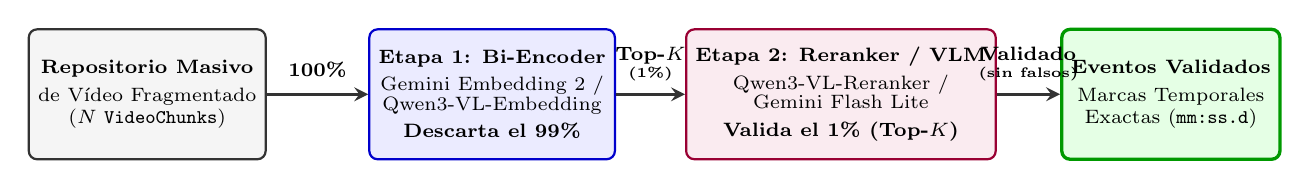
\begin{tikzpicture}[
    node distance=0.5cm and 0.6cm,
    stagebox/.style={rectangle, draw=black!80, fill=gray!8, thick, minimum width=3.0cm, minimum height=1.65cm, align=center, font=\scriptsize, rounded corners=3pt},
    resbox/.style={rectangle, draw=green!60!black, fill=green!10, very thick, minimum width=2.6cm, minimum height=1.65cm, align=center, font=\scriptsize, rounded corners=3pt},
    arrow/.style={-stealth, very thick, draw=black!80}
]
\node[stagebox] (corpus) at (-6.40, 0) {\textbf{Repositorio Masivo}\\[2pt]de Vídeo Fragmentado\\($N$ \texttt{VideoChunks})};

\node[stagebox, draw=blue!80!black, fill=blue!8, minimum width=3.1cm] (etapa1) at (-2.02, 0) {\textbf{Etapa 1: Bi-Encoder}\\[2pt]{\scriptsize Gemini Embedding 2 /}\\[-1pt]{\scriptsize Qwen3-VL-Embedding}\\[2pt]\textbf{Descarta el 99\%}};

\node[stagebox, draw=purple!80!black, fill=purple!8, minimum width=3.1cm] (etapa2) at (2.41, 0) {\textbf{Etapa 2: Reranker / VLM}\\[2pt]{\scriptsize Qwen3-VL-Reranker /}\\[-1pt]{\scriptsize Gemini Flash Lite}\\[2pt]\textbf{Valida el 1\% (Top-$K$)}};

\node[resbox] (final) at (6.60, 0) {\textbf{Eventos Validados}\\[2pt]Marcas Temporales\\Exactas (\texttt{mm:ss.d})};

\draw[arrow] (corpus) -- node[above=2pt, font=\scriptsize\bfseries] {100\%} (etapa1);
\draw[arrow] (etapa1) -- node[above=1pt, font=\scriptsize\bfseries, align=center] {Top-$K$\\[-2pt]{\tiny (1\%)}} (etapa2);
\draw[arrow] (etapa2) -- node[above=1pt, font=\scriptsize\bfseries, align=center] {Validado\\[-2pt]{\tiny (sin falsos)}} (final);
\end{tikzpicture}
\caption{Flujo del paradigma de búsqueda asimétrica en dos etapas (Regla 99\% / 1\%): el \textit{Bi-Encoder} filtra masivamente el repositorio mediante similitud del coseno en Qdrant y el \textit{Cross-Encoder} o verificador visual inspecciona únicamente el subconjunto Top-$K$ para garantizar máxima precisión con latencia mínima \cite{learnopencv_qwen3, qwen3_vl_emb2026}.}
\label{fig:embudo_asimetrico_99_1}
\end{figure}

El Cuadro~\ref{tab:comparativa_bi_cross_verificador} resume las diferencias arquitectónicas, operativas y matemáticas entre las tres familias de modelos que intervienen en el ciclo de recuperación y validación multimodal.

\begin{table}[htbp]
\centering
\small
\caption{Comparativa técnica entre arquitecturas \textit{Bi-Encoder}, \textit{Cross-Encoder} (\textit{Reranker}) y Verificadores VLM Generativos en sistemas Video RAG \cite{learnopencv_qwen3, qwen3_vl_emb2026, gemini_emb2_docs}.}
\label{tab:comparativa_bi_cross_verificador}
\begin{tabularx}{\linewidth}{>{\raggedright\arraybackslash}p{3.2cm}XXX}
\toprule
\textbf{Atributo Técnico} & \textbf{Bi-Encoder (1.ª Etapa)} & \textbf{Cross-Encoder (2.ª Etapa)} & \textbf{Verificador VLM (2.ª Etapa)} \\
\midrule
Modelos de referencia & Gemini Emb. 2 / Qwen3-Emb & Qwen3-VL-Reranker (2B/8B) & Gemini 1.5 Flash Lite / Flash 3.5 \\
Interacción Consulta-Vídeo & Tardía (Producto escalar) & Temprana (\textit{Cross-Attention}) & Generativa multimodal guiada \\
Pre-cálculo \textit{Offline} & Sí (Indexado en Qdrant) & No (Cálculo en tiempo real) & No (Evaluación bajo demanda) \\
Formato de salida & Vector $\mathbf{v} \in \mathbb{R}^d$ (MRL) & Probabilidad discreta $[0, 1]$ & Score + Justificación visual \\
Volumen procesado & $100\%$ corpus (filtra $99\%$) & $1\%$ candidatos (Top-$K$) & $1\%$ candidatos (Top-$K$) \\
Métrica optimizada & Recuerdo (\textit{Recall@K}) & Precisión (\textit{nDCG@K} / \textit{Hit@1}) & Descarte Falsos Positivos \\
\bottomrule
\end{tabularx}
\end{table}

Como demuestra esta taxonomía, la combinación de una primera etapa de vectorización densa omnimodal con una segunda etapa de atención cruzada y verificación visual constituye la arquitectura idónea para localizar eventos específicos en vídeo sin incurrir en costes computacionales prohibitivos \cite{learnopencv_qwen3, qwen3_vl_emb2026}.